\documentclass[10pt,a4paper]{article}
\usepackage[T1]{fontenc}
\usepackage[utf8]{inputenc}
\usepackage[margin=20mm]{geometry}
\usepackage{longtable,hyperref,tikz}
\usetikzlibrary{arrows.meta,positioning}
\title{HyMeKo cross-repository audit and bounded implementation}
\date{Created-at: 2026-09-05 02:57 CEST}
\begin{document}
\maketitle
\paragraph{ETA and evidence basis.} Initial baseline estimate: 45--90 minutes, including dependency builds (10--30 min), sequential tests (prior Core workspace 77 s), selected Criterion runs (10--20 min) and reporting. Expanded snapshot integration, counterexamples and the full matrix extended work beyond that initial estimate; the report records the final span. Transport uses explicitly inventoried local snapshots, not an assumed public clean-clone baseline.
\section{Scope and protected boundary}
Audit Core, Graph, Transformation/WebXR, WGPU, CUDA, Axon, Chordex and Simulator; reproduce historical measurements at their exact fixture semantics. User worktrees remain untouched. Own worktrees: \texttt{D:/hnnwork/platform-audit/\{core,graph,transformation\}}. No release, tag, main merge or push.
Protected Core items touched: empty. No Core dependency or IR/wire layout change. The precise token below authorizes two protected Graph informed-search files. Missing external governance manifests are findings; no invented authorization.
\section{Ownership and source identity}
Core \texttt{0a34a976} owns canonical Ir, compile, hash, CBOR decode/encode and generic incidence. Graph \texttt{b234c487} consumes Core and owns graph algorithms. Transformation \texttt{4298cfca} owns derived dynamics, geometry and borrowed WebXR projections; its main is stale for WebXR. Core has no WebXR production tree. Chordex owns existing byte-transparent Zenoh transport; Axon supplies deployment/bridges. Simulator owns ingress composition and presentation.
Simulator \texttt{b7a21c7} is dirty and the named ingress files are untracked; Chordex has no Git metadata. Neither is a clean-clone baseline. Audit existing state read-only; do not recreate these implementations.
\section{Affected files}
\paragraph{Approved Berge budget correction, 2026-09-05 10:45 CEST.}
The user's ``approved, continue'' reply approves the pending report proposal
\texttt{APPROVED-CORE-EDIT: graph-berge-enumeration-budget-boundaries}.
Edit only Graph \texttt{hymeko\_graph/src/direct\_ir/berge\_enum.rs} and
\texttt{hymeko\_graph/tests/direct\_ir\_optional.rs} in the clean own worktree.
Reuse the common Enumerator: a zero result cap starts stopped, after endpoint
validation. Results and expansions stop the whole search; Depth records a pruned
arc frontier while later branches continue. Test depth before charging the first
unused arc, so an exact-depth leaf with no remaining arc finishes naturally.
Global result/expansion bounds override an earlier depth marker. An unvisited arc
frontier does not prove another feasible result exists. Do not change cycle
identity, goal semantics, output ordering, public signatures, or dependencies.
Baseline: exact clean Graph 25e8c9f and Core evidence 497f18b. Reuse the prior
full-suite baseline, run current targeted tests, then run new discriminating
tests red before the production fix. Cover zero/one/exact result caps, depth
zero/exact/natural completion, later-branch results, global-bound precedence and
invalid endpoints for both paths and cycles. After the fix run the targeted and
full release suites, fmt, warning-denying Clippy, symbol and duplication checks.
Repeat the existing bounded diamond probe three times before/after on this host;
retain raw samples and resource limits. Extend the report-local summarizer for
separate before/after series and render a comparison with existing Matplotlib.
Evidence: reports/platform-audit/berge-budget-*; update the existing report,
reproducibility notes and artifact manifest without replacing historical data.
ETA: about 20--30 minutes from a cached build (prior full Graph tests 3.33 s),
including counterexample design, review and packaging. Rollback: a separate local
Graph commit on the two approved files, then its documentation commit if needed;
preserve the earlier informed-search fix and all user worktrees. No publication.
\paragraph{Approved Graph correction, 2026-09-05 03:07 CEST.}
User token: \texttt{APPROVED-CORE-EDIT: graph-directed-slots-consistent-astar}.
Additional files: Graph \texttt{hymeko\_graph/src/direct\_ir/informed.rs} and
\texttt{hymeko\_graph/tests/informed\_search\_vv.rs}.
Add a conservative default \texttt{TransitionPolicy::entry\_independent()} method
returning false; Undirected returns true. A default method preserves dyn compatibility
unlike an associated constant (review correction at 03:25 CEST). Only exit-independent costs combined with
entry-independent policy may share an arc best-entry cost. A lower g may re-expand
the arc under A*. Iterate the exact parallel incidence arc/slot slices. No existing
public function signature, canonical Core source, dependency or wire layout changes.
The three external baseline counterexamples already failed on the unchanged release
library; the existing informed diagnostic benchmark is captured before editing.
Plan bundle (this .tex, plan.tikz, plan.mmd, built plan.pdf); \texttt{reports/2026-09-05-platform-audit.md}; evidence under \texttt{reports/platform-audit/} (inventory, command logs, raw Criterion snapshots, tabular/plot results, reproducibility manifest, Graph reproducer/approval patch). Candidate non-core implementation: \texttt{hymeko\_wgpu/benches/spmm\_bench.rs}, existing \texttt{hymeko\_wgpu/tests/spmm.rs}, \texttt{tools/cuda\_prototype/spmm\_prototype.cu} and \texttt{tools/cuda\_prototype/build.sh}, only after a discriminating failure/profile. No Core public interface changes; Graph and transport additions are listed separately. Extend this file list before any additional implementation.
\paragraph{Transport implementation scope, 2026-09-05 03:29 CEST.}
Use SHA256-verified snapshots in \texttt{integration/snapshots} and clean own
worktrees in \texttt{integration/work}. Simulator's current manifest actually
selects \texttt{core-portable-id@93b1f114}; retain that exact clean revision in
an additional own worktree, separate from the audited Core benchmark revision.
Preserve sibling dependency paths with explicit directory junctions. Snapshot
Chordex, Simulator and the small auxiliary XR source; originals remain read-only.
Chordex changes: existing \texttt{src/lib.rs}, \texttt{zenoh\_backend.rs}, \texttt{tests/transport.rs},
\texttt{docs/hymeko-zenoh-contract.md}. Add a bounded latest mailbox behind the
existing CBOR subscription return type, caller-configurable payload cap (64 MiB
default), and transport-only statistics. Generic sensor FIFOs remain unchanged.
New public symbols: \texttt{DEFAULT\_MODEL\_MAX\_PAYLOAD\_BYTES},
\texttt{LatestSubscriptionStats}, \texttt{subscribe\_hymeko\_ir\_cbor\_with\_limit},
\texttt{latest\_stats}. Reject oversized samples before materializing bytes;
ignore Delete, coalesce pending Put, expose counts. This is a live mailbox,
not durable replay; reconnect uses explicit producer full-snapshot republish.
Simulator changes: existing \texttt{src/model\_ingress.rs}, \texttt{src/web.rs},
\texttt{tests/model\_ingress.rs}, \texttt{Cargo.toml}, lockfile if resolution changes.
New \texttt{from\_ir\_cbor\_if\_changed} always calls validated Core decode before
exact comparison with the bytes of the successfully installed CBOR payload.
The structural canonical hash does not cover ordinary node attributes: a capacity
2-to-3 counterexample disproved hash-only deduplication. WebViewer retains at most
one capped CBOR payload, clears it for source/UI replacements and records it only
after successful installation. A wire/hash change is not authorized or necessary.
Add
native-only optional Zenoh ingress test feature and direct test configuration
dependency using Chordex's already-resolved Zenoh 1.9; no new package family.
Local TCP tests verify meaningful dynamics/spatial state, duplicates, malformed
payloads, limits, coalescing and explicit reconnect resync. Measure null/local
transport diagnostic stages with raw samples and three runs; no new IR/codec.
Rollback is the implementation commits on these own worktrees; preserve source
snapshot commits as provenance. No claims of automatic replay or browser validation.
\paragraph{Accelerator review corrections.}
Extend existing \texttt{scripts/dev/measure\_peak\_memory.ps1}: optional direct
executable mode for the existing Rust/CUDA diagnostic probes, explicit working
directory and stdout/stderr/metric artifacts, per-child Rayon environment, and
termination during a detected RSS-limit breach. Keep the 16 GiB maximum; a lower
test cap verifies enforcement with a small child process. Record that OS high-water
counters are polled and the final poll window may be missed. Test success, nonzero
exit, redirected output and a low-limit abort; no parallel measurement framework.
The existing warm prepare benchmark accumulates unsubmitted queue writes. Replace
its cell with explicitly named prepare-plus-completion so retained staging stays
bounded; the old pure prepare number is not comparable. Gate resident correctness
before all timed cells and drop CPU expected output. Compare fresh/reused readback
in isolated, rotated processes as a control. CUDA: clamp reserved degree to columns,
check actual device launch limits before allocations, record cold setup/H2D/first
call and repeated kernel/D2H/input-to-output spans, and verify signed duplicate,
empty-row and nonfinite controls in the existing prototype. No new production backend.
\section{Execution order and gates}
\paragraph{Final bounded diagnostics and reproducibility.}
Extend the existing external Graph counterexample executable with a chain of
2, 4, 8, 12 and 16 diamonds: analytically $2^d$ simple endpoint paths, each
of length $2d$. Cap output at 4096 and expansions at one million; use a depth
limit above any simple path. Three warmups and 20 raw samples in three processes,
each supervised by the existing memory helper. Verify counts and every path
length outside the timed interval; report truncation and output steps explicitly.
Do not edit protected enumeration files. Add a small report-local Python
aggregation script and reproducibility/Kato manifest, retaining raw logs and
sample definitions. Existing diagnostics that only emit medians do not acquire
invented p95 values. Run Graph diagnostic test functions serially to avoid
cross-test contention. Record profiler permission failures without changing
device permissions. Refresh Core and Simulator SYMBOLS.md and create Graph's
missing SYMBOLS.md using existing tooling; the provider itself stays unchanged.
Consolidate duplicated test preparation in existing WGPU and external Graph test
harnesses, preserving every assertion. Render campaign PNG/SVG and an animated
trace of actual successive transport latency samples using Matplotlib already
installed on Amaterasu. This GIF is measured pipeline behavior, not browser or
simulation motion. The report-local summarizer owns all three outputs.
\paragraph{Transformation test portability correction, 2026-09-05 03:13 CEST.}
Additional files: \texttt{hymeko\_dynamics/tests/common/mod.rs} and
\texttt{hymeko\_formats/src/binary\_graph.rs} (test attributes only).
The unchanged release suite exposed two CRLF-sensitive negative-control replacements
and two debug-only panic tests executed with debug assertions disabled. Normalize CRLF
in the existing test variant helper, and gate debug-only tests explicitly. Run the
two dynamics suites in release and both format tests with debug assertions enabled.
No fixture or product behavior changes; revert these two task diffs for rollback.
\begin{enumerate}
\item Read contracts/reports, record refs/status/toolchains/dependencies/hardware. Three read-only agents investigate independently; root owns edits.
\item Compile this plan on Amaterasu using existing pdflatex, no installation. Record source and PDF hashes.
\item In clean own worktrees run locked/offline dependency audit, formatting, focused correctness and baseline tests. Classify long fault/deep-chain suites separately.
\item Reproduce directed Graph hypotheses before any optimization claim. A* uses zero or certified admissible heuristic against Dijkstra. D* deferred absent concrete dynamic use case.
\item Run Core compile/hash/CBOR/CSR and existing Graph/Transformation workloads, preserving generators and output identity. Save raw samples in three independent selected repetitions.
\item Audit accelerator oracle and separate timings. Extend existing WGPU benchmark to measure reused readback against fresh readback if justified by existing production API/profile. Do not invent a sparse incidence backend without measured need.
\item Build existing CUDA prototype with CUDA 13.2, MSVC and sm\_120; verify regular/irregular CSR and run bounded existing timing controls. These are CSR execution controls, not proven canonical-incidence semantics. Record toolkit/driver/precision/flags and profiler availability.
\item Decide C/C++ gate and Chordex ownership; document the missing end-to-end integration evidence and concrete blockers. C ABI deferred unless an actual hosted C consumer justifies it.
\item Run changed-file tests, fmt, warning-denying Clippy and contract gates, report pre-existing failures separately. Commit only named, reviewed task-owned deliverables in thematic commits.
\end{enumerate}
\section{Measurement protocol and correctness oracle}
For each run record exact SHA/branch/dirty paths, OS/CPU/RAM/GPU/driver, compiler/profile/features, relevant environment variables, input fixture/hash/seed, dimensions, precision, warmup and sample count. Do not log credentials. Criterion: at least 10 samples and 5 post-warmup observations; retain raw sample data. Report mean/median/IQR/p95/p99/worst, variance or CI; quantiles of Criterion batch averages are labelled and are not request-tail latency.
Record peak working set via Windows OS high-water counters; any sampling limitation is explicit. Maximum resident memory 16 GiB per process; monitor and terminate only task-owned processes on breach. Builds never overlap measured cells; inspect ambient processes/GPU utilization before measurement. Three repetitions when bounded; report unstable cells rather than declaring a speedup.
Core oracle: frozen canonical KAT/corpus, full decode validation/fault corpus. Graph: hand-derived minimal paths plus existing independent V\&V, identical costs/reachability and output counts. Transformation: existing physics/WebXR fixture assertions over retained canonical Core ownership. GPU: existing serial CSR oracle and documented abs/relative and NaN/Inf handling. Keep cold, prepared, resident and end-to-end metrics distinct. Retained memory is not peak RSS; structural allocation reasoning is not an allocation measurement.
\section{Backend and transport decisions}
WGPU: adapter identity includes backend/device type/driver; CPU fallback never labelled GPU. Record device/pipeline cold, allocation/upload, submitted resident work, timestamp kernel-only and readback separately; missing cells remain unmeasured.
CUDA: reuse prototype, one mathematical CSR contract, no new IR. Record setup/H2D/kernel/D2H/resident/end-to-end where instrumented; existing diagnostic timers are labelled as such. Kato runbook freezes commands and workload parameters, not cross-machine percentage comparisons.
C/C++: prefer Rust decode-backed opaque C ABI only if a consumer is identified; no new native model or schema and no automatic dual implementation.
Chordex vs Axon matrix covers charter, transport, Zenoh, dependency/runtime, QoS/backpressure, reconnect/replay/latest, ordering/duplicates, payload limits, access control, metrics and tests. Channel: existing \texttt{hymeko/model/ir/cbor/v1}; payload opaque canonical CBOR. Ordering is receiver callback arrival order, with one authorized producer per model topic; no invented sequence or timestamp. Full acceptance requires Core encode, actual local pub/sub, Core decode, Transformation projection and deterministic scene assertions, plus malformed/limit/reconnect tests.
\section{Risks, rollback and acceptance}
\paragraph{Evidence byte identity.}
Extend the existing root .gitattributes only for this dated plan, this report and
reports/platform-audit: disable text normalization so committed raw logs and
manifest SHA256 bytes match across operating systems. Package the 3022 existing
Criterion JSON files in a verified ZIP; keep unpacked local copies ignored.
Verify every archived member and every committed artifact against the manifest.
No product source attributes, dependency or provider changes. This corrects a
measured CRLF/LF mismatch in 121 artifacts during final Git-blob verification.
Worst inputs: million-incidence Core fixture, high-arity duplicate signed incidences, combinatorial Berge output, 256 MiB decoder limit and unbounded subscriber queues. Preserve output caps and never run unbounded enumeration. No benchmark output-shape change disguised as speedup. Existing stale docs, moving branch dependencies, vendor requirements and pending user changes block public reproducibility until resolved.
Rollback: task-owned feature commits and evidence only; discard/revert own changes by named path if necessary, never alter user stash, worktree or remote branches. Protected fixes require exact file list, invariant/test/rollback and one proposed approval token.
Acceptance: evidence-backed audit; historical Core values reproduced or explicitly not comparable; Graph/Transformation baselines; measured WGPU changes or justified deferral; CUDA results or runnable Kato package; C decision; Chordex decision; actual end-to-end proof or precise verified blocker; no duplicate IR/codec/WebXR; tested changes; release-readiness assessment across API/ABI/wire/docs/CI/reproducibility/fuzzing/licensing/packaging/semver. Unrun cells never pass by implication.
\section{Dependency and dataflow diagram}
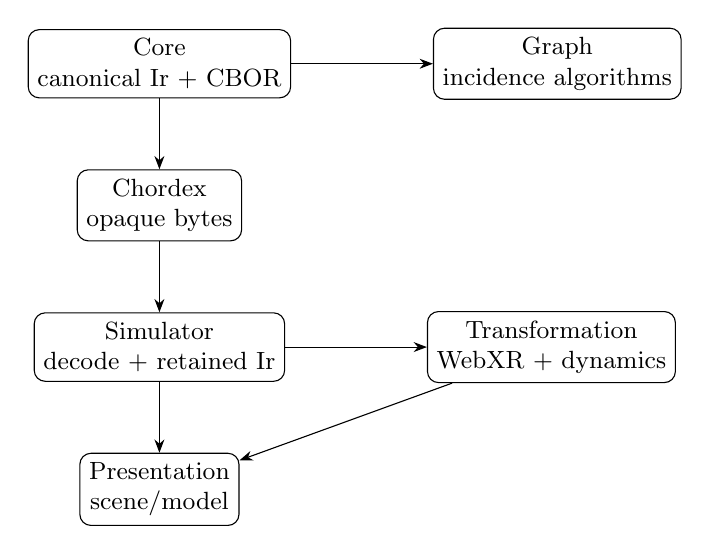
\begin{tikzpicture}[node distance=9mm, every node/.style={draw,rounded corners,align=center,font=\small},>=Stealth]
\node (core) {Core\\canonical Ir + CBOR};
\node[right=18mm of core] (graph) {Graph\\incidence algorithms};
\node[below=of core] (transport) {Chordex\\opaque bytes};
\node[below=of transport] (sim) {Simulator\\decode + retained Ir};
\node[right=18mm of sim] (trans) {Transformation\\WebXR + dynamics};
\node[below=of sim] (scene) {Presentation\\scene/model};
\draw[->] (core)--(graph);
\draw[->] (core)--(transport);
\draw[->] (transport)--(sim);
\draw[->] (sim)--(trans);
\draw[->] (trans)--(scene);
\draw[->] (sim)--(scene);
\end{tikzpicture}


\end{document}
